
\raggedright
\setlength{\parindent}{2em} %首行缩进
\newpage

\title{射影幾何自助餐} %標題
\author{Chen Xiang-Wei} %編輯這份講義的作者
\date{August 11, 2019}
\date{\today}%今天
\lfoot{Author:\theauthor}
\maketitle
\thispagestyle{fancy}
\raggedright
\rhead{模板}
\tableofcontents  % 生成目錄
%請在以下輸入內容

\setcounter{section}{-1}

\section{無窮遠炒麵線}
\pro
{\color[RGB]{0,255,200}對於}{\color{blue}複}\textbf{平}\textit{面}
~\\%空行
~\\%空行
上五點$z_{1}, z_{2}, z_{3},z_{4},z_{5}$,若\\
\[(z_{1},z_{2};z_{3},z_{4})=(z_{1},z_{2};z_{3},z_5)\]
則$z_{4}=z_{5}$\\

\subsection[short]{特殊字}

\#
\$
\%
\{
\}
\~{}
\textbackslash
\^{}


\subsection{空行的方法}

\textbackslash vspace\{1cm\}
\vspace{1cm}

\~{}\textbackslash\textbackslash
~\\%空行


\subsection{表格}
\begin{tabular}[t]{|l|c|r|}
\hline%畫一條橫線
\diagbox{c}{r} & column2 & column3 \\
\hline%畫一條橫線
item1   & item2   & item3 \\
itemA   & itemB   & itemC \\
\hline
\end{tabular}

\subsubsection*{三線表}
\begin{tabular}{cccccc}
  \toprule
  序号 & 姓名 & 性别 & 年龄 & 身高/cm & 体重/kg \\
  \midrule
  1 & 张三 & M & 16 & 163 & 50 \\
  
  \cmidrule(lr){2-3}
  \cmidrule(lr){4-5}
  \cmidrule(lr){6-6}\morecmidrules\cmidrule(lr){6-6}

  2 & 王红 & F & 15 & 159 & 47 \\
  3 & 李二 & M & 17 & 165 & 52 \\
  \bottomrule
\end{tabular}



\subsection{方框}
\fbox{
  \parbox{\textwidth}{
想法:
容易發現$HA_{PH}C_{aH}C_{aP}, HB_{PH}C_{bH}C_{bP}, HC_{PH}C_{cH}C_{cP}$是平行四邊形,\\
欲構造共圓四點$UW_aW_bW_c$使$HA_{PH},HB_{PH},HC_{PH}$分別和$UW_a,UW_a,UW_a$\\
平行且長度比例相同即可證明命題\\

  }
}

\subsection{code}

\begin{lstlisting}
  import cv2
  import mediapipe as mp
  import numpy as np
  import statistics
  import math
\end{lstlisting}

\subsection{多欄位}
\begin{multicols}{2}
  \begin{enumerate}[label=(\roman*)]
  \item 取$P$為$\Delta ABC$垂心$H$
  \item {\color{blue}取$P$為$\Delta ABC$外心$O$}
  \item {\color[RGB]{0,255,200}取$Q$為$\Delta ABC$外心$O$}
  \item 取$P$為$\Delta ABC$外接圓上一點
  \item 取$P,Q$為同一點
  \item 取$Q$為$\Delta ABC$垂心$H$
  \item 當取$P$是定點時,$Q$滿足$H,A_3,B_3,C_3$四個共圓的軌跡不超過6次
  \end{enumerate}
\end{multicols}

\subsection{Footnote}
  我是原文\footnote{我是角標}



\newpage
\section{圖片}
\begin{figure}[H]
  \centering
  \begin{minipage}[b]{0.4\textwidth} %minipage寬
  \centering
  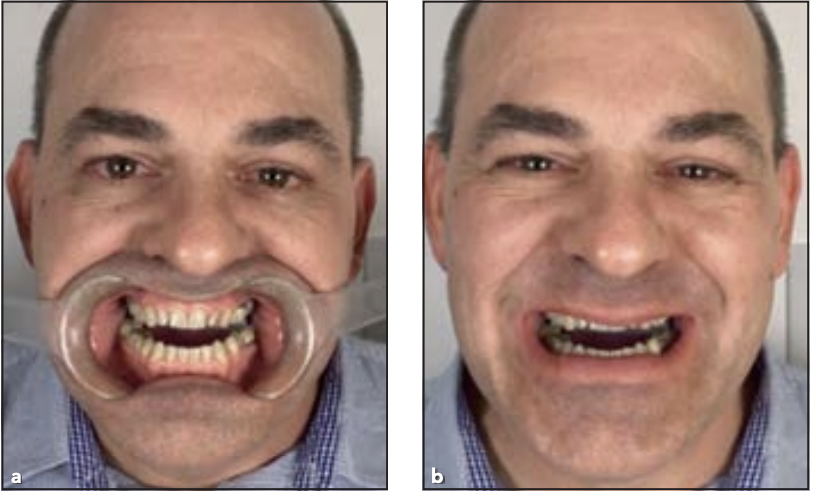
\includegraphics[width=1\textwidth]{paste_src/2023-02-07-20-49-33.png}
  \caption{正面照\upcite{dsd_tech2}}
  \label{fig:正面}
  \end{minipage}
  \begin{minipage}[b]{0.4\textwidth} %minipage宽
  \centering
  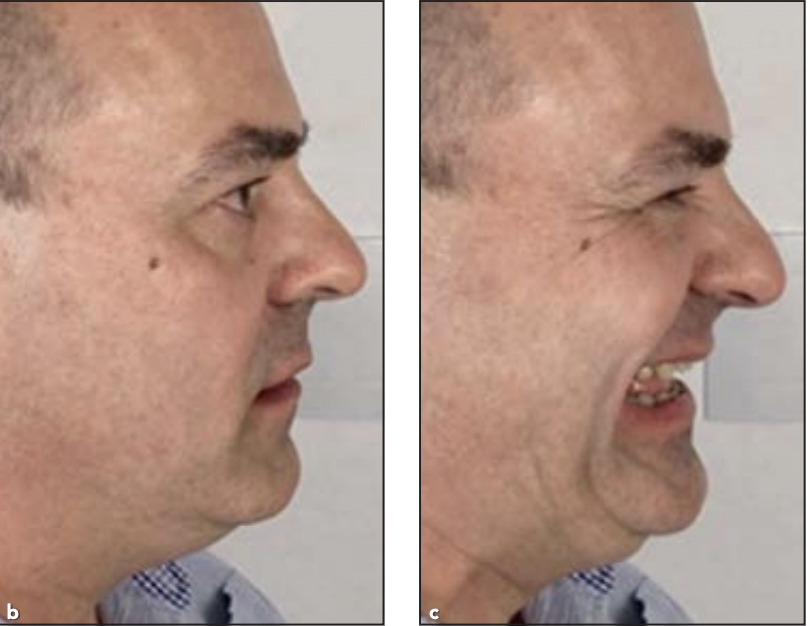
\includegraphics[width=1\textwidth]{paste_src/2023-02-07-20-50-39.png}
  \caption{側面照\upcite{dsd_tech2}}
  \label{fig:側面}
  \end{minipage}
  \end{figure}
  
\begin{figure}[H]%與文字並排
    \centering %圖片全居中
    %並排幾個圖就要開幾個minipage
    \begin{minipage}[b]{0.4\textwidth} %minipage寬
      \centering %图片局部居中
      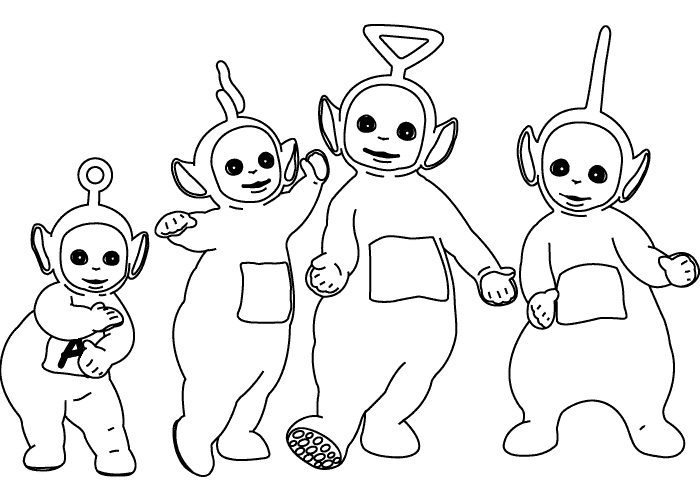
\includegraphics[width=0.8\textwidth]{a.png}
      \caption{最右邊是迪西}
      \label{fig:迪西}
    \end{minipage}
    \begin{minipage}[b]{0.4\textwidth} %minipage宽
      \centering %图片局部居中
      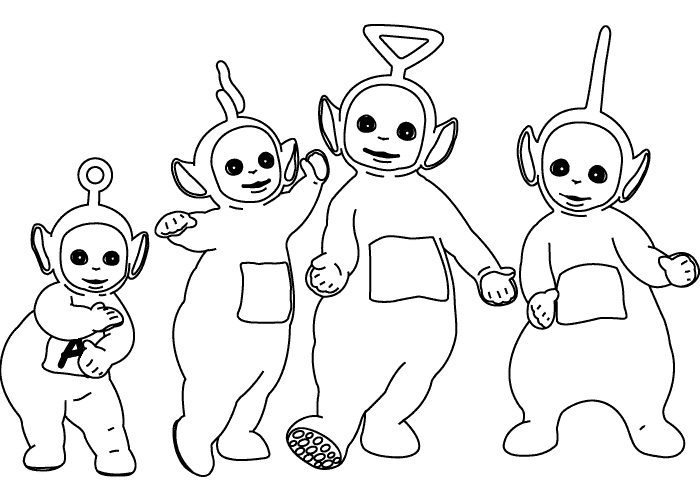
\includegraphics[width=0.8\textwidth]{a.png}
      \caption{再來是丁丁}
      \label{fig:丁丁}
    \end{minipage}
  \end{figure}
  所以
  丁丁是\prettyref{fig:丁丁}
  迪西是\prettyref{fig:迪西}




\section{My Chemical LaTeX}
  \subsection*{一些語法}
  
  \ce{2[AgCl2]-}\\
  \begin{minipage}[b]{0.3\textwidth}
    \centering
    \chemfig{*6(-=-=-=)}\\
    \chemfig{*5(-----)}\\
  \end{minipage}\\
  
  \chemfig{*6(-=-=-=)}\\
  \chemfig{*5(-----)}\\
  \chemfig{A-B}\\
  \chemfig{A=B}\\
  \chemfig{A~B}\\
  \chemfig{A>B}\\
  \chemfig{A>:B}\\
  \chemfig{A>|B}\\
  \chemfig{C(-[1]1)(-[2]2)(-[3]3)(-[4]4)(-[5]5)(-[6]6)(-[7]7)(-[0]0)}
  \ex 乙烯
  \chemfig{C(-[3]H)(-[5]H)=C(-[1]H)(-[7]H)}
  aaa

  


    

































\section{讀流程圖}

\begin{figure}[!htp]
  \centering
  \begin{tikzpicture}[node distance=2cm]

  \node (start) [startstop] {用戶透過手機app或是網頁拍攝微笑照片};
  \node (input1) [process,below of=start] {照片上傳伺服器};
  \node (process1) [process,below of=input1] {伺服器即時自動分析微笑照片};
  \node (out) [startstop,below of=process1] {將分析結果回傳到手機};


  \draw [arrow] (start) -- (input1);
  \draw [arrow] (input1) -- (process1);
  \draw [arrow] (process1) -- (out);


  \end{tikzpicture}
\end{figure}


\newpage
\tikz[remember picture,overlay] \node[opacity=0.3,inner sep=0pt] at (current page.center){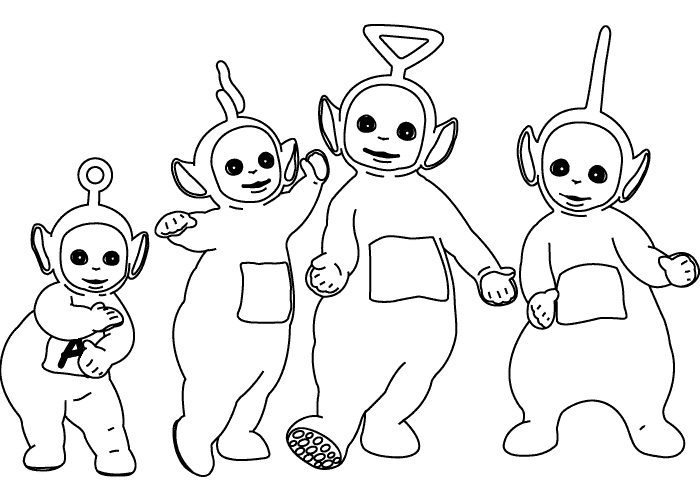
\includegraphics[width=\paperwidth,height=\paperheight]{a.png}};
\section{背景}
\subsection{tikz 實現}
編譯第一次會怪怪的,再一次就ok
\clearpage


\newpage



\AddToShipoutPictureBG*{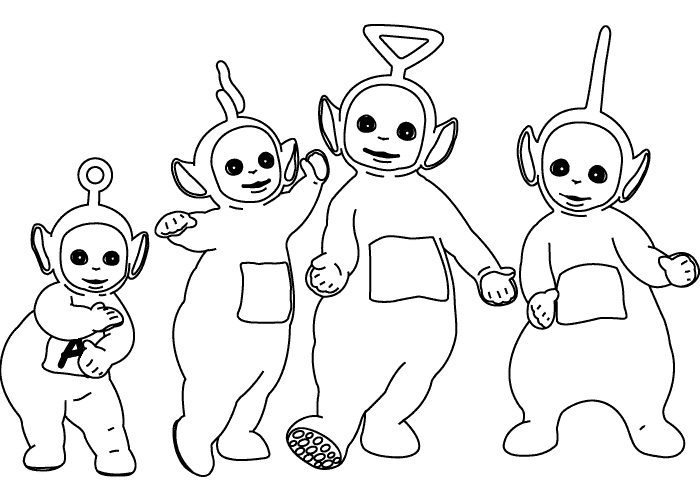
\includegraphics[width=\paperwidth,height=\paperheight]{a.png}}

\subsection{eso-pic}
text
\clearpage

\section{怪東西}
\subsection{中國象棋}

\normalboard
\begin{position}	
	\piece{a}{1}{r} \piece{i}{1}{r}
	\piece{b}{1}{n} \piece{h}{1}{n}
	\piece{c}{1}{b} \piece{g}{1}{b}
	\piece{d}{1}{g} \piece{f}{1}{g}
	\piece{e}{1}{k}
	\piece{a}{4}{p} \piece{c}{4}{p}	\piece{e}{4}{p} \piece{g}{4}{p}	\piece{i}{4}{p} 
	\piece{b}{3}{c} \piece{h}{3}{c}		
	\piece{a}{10}{R} \piece{i}{10}{R}
	\piece{b}{10}{N} \piece{h}{10}{N}
	\piece{c}{10}{B} \piece{g}{10}{B}
	\piece{d}{10}{G} \piece{f}{10}{G}		
	\piece{e}{10}{K}
	\piece{b}{8}{C} \piece{h}{8}{C}
	\piece{a}{7}{P} \piece{c}{7}{P} \piece{e}{7}{P} \piece{g}{7}{P} \piece{i}{7}{P} 	
\end{position}

\bibliography{bibfile} 
\bibliographystyle{unsrt}
